\documentclass[11pt,a4paper]{report}

\usepackage{url}
\usepackage[utf8]{inputenc}
\usepackage{graphicx}
\usepackage[all]{xy}
\usepackage{amsmath}
\usepackage{amsthm}
\usepackage{amssymb}
\usepackage{todonotes}
\usepackage{array}
\usepackage{listings}
\usepackage{hyperref}
\usepackage{tikz}
\usepackage{graphicx}  
\usepackage[toc,page]{appendix}
\usepackage[a4paper]{geometry}

\usetikzlibrary{matrix,shapes,arrows,positioning,chains,calc}

\makeatletter %otherwise geometry resets everything
\Gm@restore@org
\makeatother

\setlength{\itemsep}{0cm}
\setlength{\voffset}{0cm}
\setlength{\headheight}{0cm}
\setlength{\topmargin}{0cm}
\setlength{\extrarowheight}{3pt} %for superscripts in tabular
\setlength{\arraycolsep}{4pt}
\lstset{basicstyle = \footnotesize, breaklines = true}

\graphicspath{{imgs/}}

\begin{document}
\begin{titlepage}
\begin{center}
\textsc{\LARGE Bachelor thesis\\Computer Science}\\[1.5cm]

\includegraphics[height=100pt]{logo}

\vspace{0.4cm}
\textsc{\Large Radboud University}\\[1cm]
\hrule
\vspace{0.4cm}
\textbf{\huge Inferring state machines of Tunneled Direct-Link Setup}\\[0.4cm]
\hrule
\vspace{2cm}
\begin{minipage}[t]{0.45\textwidth}
\begin{flushleft} \large
\textit{Author:}\\
S\'ebastiaan Versteeg\\
s4459636\\
\texttt{hello@sebastiaan.app}\\
\end{flushleft}
\end{minipage}
\begin{minipage}[t]{0.45\textwidth}
\begin{flushright} \large
\textit{First supervisor/assessor:}\\
dr. ir. Joeri de Ruiter\\
\texttt{joeri@cs.ru.nl}\\[1.3cm]
\textit{[Second supervisor:]}\\
title, name\\
\texttt{e-mail address}\\[1.3cm]
\textit{Second assessor:}\\
title, name\\
\texttt{e-mail address}
\end{flushright}
\end{minipage}
\vfill
{\large \today}
\end{center}
\end{titlepage}

\begin{abstract}
The abstract of your thesis is a brief description of the research hypothesis,
scientific context, motivation, and results.
The preferred size of an abstract is one paragraph (\textit{``alinea"}) or one page of text.
\end{abstract}


\tableofcontents
\chapter{Introduction}\label{introduction}

\iffalse
The introduction of your bachelor thesis introduces the research area, the
research hypothesis, and the scientific contributions of your work.
A good narrative structure is the one suggested by Simon Peyton Jones
\cite{80211}:
%
\begin{itemize}
\item describe the problem / research question
\item motivate why this problem must be solved
\item demonstrate that a (new) solution is needed
\item explain the intuition behind your solution
\item motivate why / how your solution solves the problem (this is technical)
\item explain how it compares with related work
\end{itemize}
\fi


A lot has changed since the introduction of personal computers. Networks have been set-up everywhere and smartphones have been invented. With the introduction of new technologies also came the interest into the protection of data sent using the internet. The most used wireless internet protocol is defined in the 802.11 specification \cite{80211} and is more commonly known as ‘Wi-Fi’. Part of this specification is a way to let clients (stations, STAs) communicate without severing the connection to the shared access point (AP), this is called a Tunneled Direct Link Set-up (TDLS).  This specific part of the specification introduces a protocol handshake which is used to secure the link. We want to look into this part of the specification, analyse the implementation to find out if this handshake is properly executed. Since the protocol is intended for public use, people should be able to rely on the handshake to be completely secure. Analysing the implementation will make sure the public can use the TDLS functionality without worrying about how secure their connection is. The analysis executed in this thesis will use the learning algorithm L* to infer the state machine of the TDLS implementation. This state machine will be checked by using the algorithm randomwords. To create the packets used during the inferring we will use a mapper written in Python using ScaPy.

This thesis is structured as follows: firstly we will discuss the TDLS protocol and the 802.11 specification. Next we will take a look at Mealy machines and how to infer that kind of state machines using the previously mentiond algorithms. Consequently we will explain how we implemented our mapper and how it works in our setup. Lastly we will analyse the inferred state machines by comparing them to the specification.
\chapter{Preliminaries}\label{preliminaries}

In this chapter we give an introduction to the protocol and method we're using for our research.

\section{Tunneled Direct-Link Setup}\label{tdls}

\iffalse
- TDLS
	- 802.11
	- PeerKey
\fi

\subsection{General}

Tunneled Direct-Link Setup (TDLS) is a part of the IEEE 802.11 specification\cite{80211} that allows two devices to create a direct connection. This specification is more commonly known as Wi-Fi and allows devices to establish a wireless local area network.

A 802.11 network exists of one or more stations (STAs). A usual setup has one station that operates as access point (AP). All other stations connect to that AP and use it as the gateway for their data. TDLS allows stations connected to the AP to simultaneously set up a direct link between two stations. This reduces the amount of traffic transferred via the access point and avoids congestion inside that access point.

\subsection{Establishing a direct-link}
\label{sec:establishing-tdls}

To establish a direct-link we need two stations. One of the stations is called the \emph{initiator}, the other is the \emph{responder}. The messages they use to manage their connection are shown in figure \ref{fig:establishment-mcs}. The first message in the exchange to establish a new link is send through the access point by the initiator to the responder, who proposes a direct-link based on similar capabilities of the two stations. The responder replies through the access point either with a status code indicating success or failure in the setup response. The receival of this message is then confirmed by the last message in this part of the exchange. If any of the two stations wants to sever the direct link they can do this by sending a teardown message. This teardown message can both be send through the access point or directly to the receiving station.

\begin{figure}[!h]
	\centering
	\includegraphics[height=200pt]{estmcs}
	\caption{The TDLS direct-link establishment}
	\label{fig:establishment-mcs}
\end{figure}

\subsection{TDLS PeerKey}
\label{sec:tdls-peerkey}

A direct link connection can be secured via the TDLS PeerKey (TPK). This handshake establishes a Robust Secure Network Associaton (RSNA) for the direct link. The generated TPK in this handshake is used to provide data origin authenticity of the setup messages and the confidentiality for data that will be send over the direct link.

The handshake is a part of the messages used to establish a direct link. Fields from these messages are used to calculated the TPK and consequently to calculate a Message Integrity Code (MIC).

The fields used in the calculation of the TPK are two nonces (SNonce and ANonce) and the MAC addresses of the initiator, responder and access point. The handshake (figure \ref{fig:tpk-mcs}) is started by the initiator who sends a chosen ciphersuite (RSNE) and the SNonce to the responder station. The responder will use its own nonce to generate the TPK. This TPK is then used to calculate the MIC with the whole message as input. The initiator, who is now receiving both the nonces and a calculated MIC will derive the TPK as well and confirm that the MIC is valid. The responder will then send the 3rd message containing a new MIC to validate the direct link.

\begin{figure}[!h]
	\centering
	\includegraphics[height=140pt]{tpkmcs}
	\caption{The TPK Handshake}
	\label{fig:tpk-mcs}
\end{figure}
\section{Model Learning}\label{modellearning}

\subsection{Mealy machines}

To model the implementation of TDLS we're going to use a specific kind of state machine, \emph{Mealy machines}. This type of state machine is a kind of deterministic finite state machine that has a transition and output for every state and input \cite{Mealy:1955}.

A Mealy machine is formed by a set of finite states (\(Q\)) and the transitions between those states. One of these states is the initial state \(q_0\), the state where the Mealy machine always starts. Transitions represent an input received while the machine is one of the its states. The transitions are defined as \(\delta : Q \times \Sigma \to Q\). This function uses the input alphabet \(\Sigma\), which is a finite set of symbols that represent the input. Different from a normal finite state machine is the output function \(\lambda = Q \times \Sigma \to \Lambda\) where \(\Lambda\) is the finite set of output symbols.

Since a Mealy machine is deterministic the state machine has only one transition for each input. This is perfect for our research since TDLS should reply the same every time the same message sequence is executed.

\begin{figure}[!h]
	\centering
	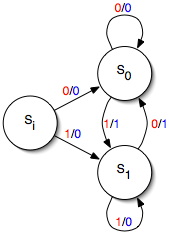
\includegraphics{mealy}
	\caption{Example of a Mealy machine}
	\label{fig:mealymachine}
\end{figure}

\subsection{Learning state machines}

Our goal is to learn a state machine of a TDLS implementation. We're approaching this by using the L* algorithm \cite{Angluin:1987}. The goal of this algorithm is to learn a finite state machine from a so-called \emph{teacher}. This teacher can be any type of computational system.
The L* algorithm is run by the learner, who tries to communicate with the teacher to infer the state machine of that teacher. In our learning process this teacher will be an implementation of TDLS.

\subsubsection{Learning process}

The first step in the learning process is sending arbitrary messages to the teacher. The teacher will answer based on the message sent by the learner. These answers can differ for each type of message sent by the learner. This allows the learner to build a hypothetical state machine based on those messages, both the input and output.
Since the state machine of the learner is only hypothetical it needs needs to check with the teacher if it matches the actual state machine.

Checking if the state machines match is done by using an equivalence algorithm, in our case we choose to use \emph{randomwords}. This algorithm will send a random sequence of inputs of a predefined minimum and maximum length to the teacher. If the output of the teacher based on this input matches the inferred state machine the next sequence of input will be sent. After a predefined number of tries the learner will draw the conclusion that the inferred state machine is equal to the state machine of the teacher. If the output of the teacher does not match the state machine the learner will know based on the response, it will then try inferring a new state machine.


\section{Tooling}

\subsection{LearnLib}

The first of the tools used to execute our research is LearnLib \footnote{https://learnlib.de/}. This is, as they call it, "an open framework for automata learning". It is free and open source under the Apache 2.0 License. The development is executed at the Char for Programming Systems of TU Dortmund University in Germany, where it was introduced by Malte et al. \cite{Malte:2015}. 
LearnLib features both multiple learning algorithms and multiple strategies to approximate equivalence, of which L* and random words are used in this thesis.
The version used in this thesis, 0.12.0, was released in June 2015. The latest version (0.13.1) was released in May 2018 since development was picked up again. However, since we're not using LearnLib directly but via StateLearner we're not able to use the latest version.

\subsection{StateLearner}

The second tool is called StateLearner \footnote{https://github.com/jderuiter/statelearner}, developed by Joeri de Ruiter. This tool is based on LearnLib and is tailored to automated model learning. It connects to the implementation of the subject either directly or via a mapper. In our case a mapper takes the symbols of the input alphabet that we provide StateLearner with and maps those symbols to the appropriate messages. The responses are then once again mapped to symbols that form the output alphabet. This way we can use StateLearner to form hypotheses using LearnLib.
\chapter{Research}\label{research}

This chapter will explain the setup used to infer the state machine of a TDLS implementation.
We will take a look at the mapper, which is used to convert input and output symbols used by StateLearner to the right TDLS messages. Next we will focus on the assumptions made for this research, plus the final setup used.

\section{Mapper}

As previously mentioned StateLearner requires a mapper to send and receive messages to the TDLS implementation. First we'll explore two tools used in our mapper: Scapy and pycrypto. Then we will look how these tools are used in our mapper.

\subsection{Scapy}

Scapy \footnote{https://github.com/secdev/scapy} is a Python program that allows you to capture, manipulate and send network packets. This open source library was used to create the 802.11 TDLS packets and wrap them inside Ethernet frames. Scapy itself has support for the basic 802.11 packets that are part of the specification. The 802.11 specification actually identifies packets as a piece of base information, the action that should be executed and so-called elements that can differ based on the action requested. Scapy implements packets that could be used for the normal 4-way handshake, but it does not implement any TDLS messages.
This means that we implemented the complete messages used for TDLS from scratch using the building blocks that Scapy provides. This includes the Setup Request, Setup Response, Setup Confirm and Teardown messages that we previously discussed in section \ref{sec:establishing-tdls}.

\subsection{Cryptographic utilities}

The construction of TDLS messages involves cryptographic operations. These operations, hashing algorithm SHA256 and the AES encryption algorithm are not natively implemented in Python itself, therefore we need an external implementation. The solution we're using for our research is the Python Cryptography Toolkit \footnote{https://github.com/dlitz/pycrypto} or pycrypto for short. This toolkit, also open-source, implements multiple secure hash functions and various encryption algorithms and it has been used in this type of research before \cite{Vanhoef:2017,Veldhuizen:2017}.

\subsection{Implementation}
\label{research:mapper:implementation}

The implementation of the mapper was written in Python to make use of the previously mentioned tools. It exposes a socket connection to the learner to enable communication between the mapper and the learner. The input symbols determined by the learner are sent over the socket and transcribed into the right TDLS messages. These messages are then send on the network interface of the learner side in the network.
The side of the teacher gets the time to answer and the mapper will subsequently translate the answer to the right output symbols. The output symbol will then be send back to the learner and the mapper will be made ready for the next input symbol. If the mapper receives a setup response message from the implementation the contents of the message will be saved in the mapper. This message contains the ANonce, SNonce, BSSID and MAC addresses needed to create the right TPK for the connection. That TPK is used if the next message by the learner is a setup confirm message. Any other symbol, except for the connection check, from the learner will reset these values.

Since it is not possible to check if a TDLS connection is made the mapper assumes a successful connection and disconnection after a correct handshake and a sent teardown respectively. The initialisation of a new connection will also assume a disconnect, as per the specification. We have tried to send pings over the TDLS connection to confirm a successful setup, but the virtual interfaces did not seem to support this usage. Another solution we tried was doing a TDLS channel switch, however the interface does not offer this functionality as well. This exhausted our options to test the connection, so we settled on keeping an internal state.

Our input alphabet exists of the following symbols: 
\begin{itemize}
	\item SETUP\_REQUEST - Translates to a TDLS setup request message
	\item SETUP\_CONFIRM - Translation to a TDLS setup confirm message
	\item TEARDOWN - Translates to a TDLS teardown message
	\item CONNECTED - Translates to the internal mapper connection status
\end{itemize}

The output alphabet is defined as follows:
\begin{itemize}
	\item SETUP\_RESPONSE - Translation from a successful TDLS setup response message
	\item NO\_RESPONSE - Indicates that no response was received
	\item CONNECTED - Indicates that the mapper detected a completed setup
	\item NOT\_CONNECTED - Indicatest that the mapper has not detect a completed setup
\end{itemize}


\section{Setup}

\subsection{wpa\_supplicant}

The implementation we used for our research is the wpa\_supplicant\footnote{https://w1.fi/} software written by Jouni Malinen. This Linux user space 802.11 client is used in all major Linux distributions and mobile operating system Android.
Along with wpa\_supplicant comes the access point software called hostapd. We do not look at it's implementation but it will serve as virtual access point during our testing of wpa\_supplicant. Our research could be conducted with any type of access point.

We will use version 2.7 of hostapd and wpa\_supplicant to conduct our research. This version was released in December 2018.

\subsection{Networking}

Before we can run the mapper and learner to infer the state machine we'll have to setup a simulated network environment. Since the wpa\_supplicant/hostapd source code already includes automated tests that use such a simulated environment we'll be partially reusing this implementation.
The environment requires a special build of both wpa\_supplicant and hostapd which can be constructed by following the instructions in the repository \cite{Malinen:2013}.
Our test will use the mac80211\_hwsim Linux kernel driver which is capable of simulating 802.11 hardware. We setup three interfaces: one WPA2 protected access point and two stations. The access point is running hostapd, the stations are controlled by wpa\_supplicant. Since we know the MAC addresses of the access point and both stations we're able to craft messages and send them via the AP to the receiving wpa\_supplicant instance. The response of that instance can then be read by sniffing the interface of the interface we simulated to be the sender.

\begin{figure}[!h]
	\centering
	\includegraphics[width=\textwidth]{setup}
	\caption{A visual representation of our setup}
	\label{fig:setup}
\end{figure}


\chapter{Results}

In this chapter we state our expectations of the inferred model. Next we evaluate the results of the learner by comparing them to our expectations using a manual analysis.

\section{Expectations}

We expect that the TDLS state machine has three states:
\begin{enumerate}
	\item No TDLS connection
	\item Setup in progress
	\item Active TLDS connection
\end{enumerate}

If we follow the 802.11 specification we should have at least the following edges:
\begin{itemize}
	\item State 0 to 1: TDLS Setup Request resulting in a TDLS Setup Response with status code SUCCESS (\cite[11.23.4]{80211})
	\item State 1 to 2: TDLS Setup Confirm without response
	\item State 2 to 0: TDLS Teardown without response
	\item State 2 to 1: TDLS Setup Request resulting in a TDLS Setup Response (11.23.4 sub e \cite{80211})
\end{itemize}

Since we do not get a response from all requesting messages the mapper will, as previously mentioned, make assumptions on the status of the connection. This means that every state will also have an edge indicating the status.

\section{Analysis}

The state machine learned by the L* algorithm does not deviate from the previously mentioned requirements of the implementation. It has more edges than mentioned. These edges would not cause any differences, since the state stays the same. This is a reflection from the specification, without the current message order no action should be taken. However, that the state machine is not different may be influenced by the assumption made by the mapper. Since we could not find a working procedure to check if a TDLS connection was setup successfully this was to only way to obtain a seemingly valid model.

\section{Interesting findings}

\begin{enumerate}
	\item WPA supplicant tests do not really rely on communication to check a tdls connection
	\item No support for channel switch in hwsim
	\item No response from interface at all, may be driver is the issue?
\end{enumerate}

\chapter{Related Work}\label{relatedwork}
\iffalse
In this chapter you demonstrate that you are sufficiently aware of the
state-of-art knowledge of the problem domain that you have investigated as
well as demonstrating that you have found a \emph{new} solution / approach / method.

TODO: Add paper by Joeri.
Bachelorthesises by Jules, Bart, Max
State machines in network and security protocols
Wi-Fi stuff
\fi

In this chapter we give an overview of all previous work related to the security of Wi-Fi and/or the use of models to test or infer state machines.

\subsection{Wi-Fi}

The authentication of clients with access points within the 802.11 specification, Wi-Fi, is facilitated by the so-called 4-way handshake. Closely related to this thesis is the research into both the manual \cite{Vanhoef:2017} and automated \cite{Stone:2018} state learning of that handshake.

The 4-Way Handshake has also been subject of numerous formal analyses \cite{He:2004,Dong:2009,Xing:2008,He:2005}. Other parts of 802.11, but related to the 4-way handshake, that have been the subject of research are the WEP and WPA2 TKIP security mechanisms \cite{Fluhrer:2001,Vanhoef:2013}.

More in-depth research into the handshake discovered a vulnerability in the transmission of the group-key \cite{Vanhoef:2016}. This research by Vanhoef et al. forced RC4 encryption of the group key, which is insecure \cite{Fluhrer:2001}. Following this discovery Vanhoef et al. introduced an attack that reinstalls the key used by the 4-way handshake making replaying, decryption and forging of packets possible \cite{Vanhoef:2017-2}.

We are not aware of any previous work on the Tunneled Direct-Link Setup functionality of the 802.11 specification.

\subsection{Learning state machines}

Past work relying on state machine learning has already been mentioned in the previous section. Both the manual and automated modeling of the 4-way handshake \cite{Vanhoef:2017,Stone:2018}. However, there is other research that analyses protocols by inferring the state machines. Aarts et al. \cite{Aarts:2013} used model-based learning to infer to state machines of EMV cards. Additionally, hand-held readers use for internet banking were subject of research \cite{Chalupar:2014} along with the TLS protocol \cite{Ruiter:2015,Thoor:2018}. These analyses discovered several security flaws in different implementations of TLS. Other implementations of protocols analysed via this technique are SSH \cite{Brostean:2017,Tijssen:2015} and IPSec \cite{Veldhuizen:2017}.

Furthermore, the technique was also used for a non-security related subject by learning the TCP network protocol \cite{Brostean:2014}. This revealed ways to fingerprint remote operating systems.
\chapter{Future work}
\label{futurework}

Our research can be used a basis for future investigation into this topic. We will point out several possiblities.

In our research we have not taken error messages or timeouts into account. This was to simplify our research. Better results may be found when these factors are introduced. One of the ways to do this would be to use an improved version of the StateLearner\footnote{https://github.com/ChrisMcMStone/statelearner} software that we used. 
Related to this improved would be changing the values of the messages that are send using the mapper, more commonly known as fuzzing. Using this method we might be able to find states that we currently did not find. This should be considered since fuzzing would introduce error responses to the mapper. The learner will thus learn about the different variations of responses.
Lastly we could execute this research on real hardware instead of using a simulated environment. This would introduce more new factors: packet loss and interference. It might however be able to use the TDLS channel switch to confirm a successful connection. This would greatly improve the resulting model.
\chapter{Conclusions}\label{conclusions}
\iffalse
In this chapter you present all conclusions that can be drawn from the
preceding chapters.
It should not introduce new experiments, theories, investigations, etc.:
these should have been written down earlier in the thesis.
Therefore, conclusions can be brief and to the point.
\fi

In this research we've shown that this method of inferring the TDLS state machine is not ideal. This does not mean that this method is not useful for researching protocols.
Future work is required to come to a better understanding of the TDLS state machine implementations.

\bibliographystyle{plain}
\bibliography{bibliography}

\begin{appendices}
\chapter{State Machine Models}\label{appendix:a}

\begin{figure}[!h]
	\centering
	\includegraphics[height=0.9\textheight]{fullModel}
	\caption{Full TDLS State Machine}
	\label{fig:tdls-sm-full}
\end{figure}

% \begin{figure}[!h]
% 	\centering
% 	\includegraphics[height=0.9\textheight]{cleanedModel}
% 	\caption{Cleaned TDLS State Machine}
% 	\label{fig:tdls-sm-cleaned}
% \end{figure}
\end{appendices}

\end{document}
